\documentclass[11pt]{article}
\def\nterm {}
\def\nyear {2022 - 2023}
\def\nlecturer {A. Veraart, D. Bodenham}
\def\ncourse {Probability and Statistics}
\def\nshort {Probability and Statistics}
\usepackage{amsmath, amsthm, amssymb, amsfonts}
\usepackage{fancyhdr}
\usepackage{xparse, xpatch}
\usepackage[svgnames]{xcolor}
\usepackage[shortlabels]{enumitem}
\usepackage[thinc,text]{esdiff}
\usepackage[bottom]{footmisc}
\usepackage[most]{tcolorbox}
\usepackage{physics}
\usepackage{tikz}
\usepackage{pgfplots}
\usepackage{graphicx, tabularx, caption}
\usepackage{csquotes}
\usepackage[a4paper, left=1.2in, right=1.2in, bottom=1in]{geometry}
\usepackage[hidelinks]{hyperref}
\hypersetup{
    colorlinks,
    allcolors=black
}
\pgfplotsset{compat=1.18}
\graphicspath{{./images/}}

% meta
\setlength{\headheight}{13.6pt}
\renewcommand*\contentsname{Outline}
\pagestyle{fancy}
\lhead{\nouppercase{\leftmark{}}}
\rhead{\nshort}
\title{\textbf{\ncourse}}
\author{Lectured by \nlecturer \\\small Notes taken by Dongshen Wu\footnote{These notes are usually modified significantly after lectures, and are not endorsed by the lecturers at Imperial College, London. They are by no means an accurate representations of what was actually lectured. In particular, all errors are almost surely mine.}}
\date{\nterm \nyear}

% centre tikz pictures
\makeatletter
\g@addto@macro\@floatboxreset\centering
\makeatother

% environment
\tcbset{
  defstyle/.style={
    enhanced, sharp corners,
    attach boxed title to top left={yshift=-2.75mm, 
      xshift=5mm, yshifttext=-2.2mm},
    colback=white, colframe=PeachPuff,
    coltitle=black, fonttitle=\bfseries,
    before skip=7pt,
    boxed title style={sharp corners, size=small,
      colback=PeachPuff,colframe=PeachPuff,}},
  thmstyle/.style={
    enhanced, sharp corners,
    attach boxed title to top left={yshift=-2.75mm, 
      xshift=5mm, yshifttext=-2.2mm},
    colback=AliceBlue, colframe=LightBlue,
    coltitle=black, fonttitle=\bfseries,
    before skip=7pt,
    boxed title style={sharp corners, size=small,
      colback=LightBlue,colframe=LightBlue,}},
  propstyle/.style={
    enhanced, sharp corners,
    attach boxed title to top left={yshift=-2.75mm, 
      xshift=5mm, yshifttext=-2.2mm},
    colback=white, colframe=PowderBlue,
    coltitle=black, fonttitle=\bfseries,
    before skip=7pt,
    boxed title style={sharp corners, size=small,
      colback=PowderBlue,colframe=PowderBlue,}},
}

\newtcbtheorem[number within=section]{TcbThm}{Theorem}{
  thmstyle}{thm}
\NewDocumentEnvironment{theorem}{ O{} O{} }
  {\TcbThm{#1}{#2}}{\endTcbThm}

\newtcbtheorem[number within=section, use counter from=TcbThm]{TcbProp}{Proposition}{
  propstyle}{prop}
\NewDocumentEnvironment{proposition}{ O{} O{} }
  {\TcbProp{#1}{#2}}{\endTcbProp}

\newtcbtheorem[number within=section,use counter from=TcbThm]{TcbDef}{Definition}{
  defstyle}{def}
\NewDocumentEnvironment{definition}{ O{} O{} }
  {\TcbDef{#1}{#2}}{\endTcbDef}

\newtcbtheorem[number within=section,use counter from=TcbThm]{TcbAxi}{Axiom}{
  defstyle}{axi}
\NewDocumentEnvironment{axiom}{ O{} O{} }
  {\TcbAxi{#1}{#2}}{\endTcbAxi}

\newtheorem{corollary}[\tcbcounter]{Corollary}
\tcolorboxenvironment{corollary}{propstyle}
\newtheorem{lemma}[\tcbcounter]{Lemma}
\tcolorboxenvironment{lemma}{propstyle}

\theoremstyle{definition}
\newtheorem*{example}{Example}
\newtheorem*{exercise}{Exercise}
\newtheorem{problem}{Problem}
\newtheorem*{algorithm}{Algorithm}
\newtheorem*{procedure}{Procedure}
\newtheorem*{remark}{Remark}
\tcolorboxenvironment{algorithm}{propstyle}

\theoremstyle{remark}
\newtheorem*{notation}{Notation}
\newtheorem*{solution}{Solution}
\tcolorboxenvironment{solution}{
  blanker,breakable,left=5mm,
  before skip=10pt,after skip=10pt,
  parbox = false,
  borderline west={0.5mm}{0pt}{SlateGray}}
\tcolorboxenvironment{proof}{
  blanker,breakable,left=5mm,
  before skip=10pt,after skip=10pt,
  parbox = false,
  borderline west={0.5mm}{0pt}{SlateGray}}

\newtcolorbox{extension}[1]{
  colback=WhiteSmoke,colframe=Gainsboro, enhanced, before skip=10pt, after skip=10pt, fonttitle=\bfseries,coltitle=black, sharp corners, title={\:\,Extension:\:#1}, before upper app={\setlength{\parindent}{17pt}}
}

% subproof
\makeatletter
\newcounter{subproof}
\xpretocmd{\proof}{\setcounter{subproof}{0}}{}{}
\xpretocmd{\solution}{\setcounter{subproof}{0}}{}{}
\newcommand{\subproof}[1]{%
  \par
  \addvspace{\medskipamount}%
  \stepcounter{subproof}%
  \noindent\emph{Part \thesubproof: #1}\par\nobreak
  \@afterheading
}
\makeatother

% command
\newcommand{\C}{\mathbb{C}}
\newcommand{\N}{\mathbb{N}}
\newcommand{\Q}{\mathbb{Q}}
\newcommand{\R}{\mathbb{R}}
\newcommand{\Z}{\mathbb{Z}}
\renewcommand{\bf}[1]{\mathbf{#1}}
\renewcommand{\cal}[1]{\mathcal{#1}}
\renewcommand{\rm}[1]{\mathrm{#1}}
\newcommand{\floor}[1]{\left \lfloor #1 \right \rfloor}
\newcommand{\ceil}[1]{\left \lceil #1 \right \rceil}
\newcommand{\lointerval}[1]{\ensuremath{\left(#1\right]}}
\newcommand{\rointerval}[1]{\ensuremath{\left[#1\right)}}
% Augmented Matrix
\newenvironment{amatrix}[1]{%
  \left(\begin{array}{@{}*{#1}{c}|c@{}}
}{%
  \end{array}\right)
}

\begin{document}
\maketitle{}
\tableofcontents{}
\pagebreak
%=========================================================
\part{Probability}
\section{Counting}
\subsection{Sample space}
\begin{definition}[Sample space]
  The sample space \(\Omega\) is the set of all possible outcomes of an experiment. The elements of \(\Omega\) are sample points, typically denoted as \(\omega\). Subsets of \(\Omega\) are events.
\end{definition}

We see from this definition that probability theory is based on set theory. For instance, \(\emptyset \subseteq A \subseteq \Omega\) implies the probability of an event is between 0 and 1. It is therefore useful to remind ourselves with some useful laws we learnt in IUM.

\begin{proposition}[De Morgan's and Distributive]
  Let \(\mathcal{I}\) be a general index set. Suppose \(A_i \subseteq \Omega, \forall i\in \mathcal{I}\) and \(B\subseteq \Omega\). Then,
  \begin{itemize}
    \item De Morgan's laws: 
    \begin{align*}
      \left(\bigcap_{i\in\mathcal{I}}A_i \right)^\complement
      &= \bigcup_{i\in\mathcal{I}}A_i^\complement
      & \text{and}& 
      & \left(\bigcup_{i\in\mathcal{I}}A_i \right)^\complement &= \bigcap_{i\in\mathcal{I}}A_i^\complement
    \end{align*}
    \item Distributive laws:
    \begin{align*}
      B \cap \left(\bigcup_{i\in\mathcal{I}}A_i \right)
      &= \bigcup_{i\in\mathcal{I}}(B \cap A_i)
      & \text{and}& 
      & B \cup \left(\bigcap_{i\in\mathcal{I}}A_i \right)
      &= \bigcap_{i\in\mathcal{I}}(B \cup A_i)
    \end{align*}
  \end{itemize}
\end{proposition}

A general strategy to prove equality of set is to pick an arbitrary elements \(x\) and shows that \(x\in A \iff x \in B\).
\begin{proof}
  \subproof{De Morgan's}
  Let \(x \in \left(\bigcap_{i\in\mathcal{I}}A_i \right)^\complement\) be arbitrary. This means that \(x\) is not in all \(A_i\). Hence there exists at least one \(j \in \mathcal{I}\) such that \(x \notin A_j\), i.e. \(x \in A_j^\complement \subseteq (\bigcup_{i\in\mathcal{I}}A_i^\complement)\).

  Let \(x \in (\bigcup_{i\in\mathcal{I}}A_i^\complement)\). This means there exists at least one \(j \in \mathcal{I}\) such that \(x \in A_j^\complement\), i.e. \(x \notin A_j\). Thus, \(x \notin (\bigcap_{i\in\mathcal{I}}A_i)\), i.e. \(x \in (\bigcap_{i\in\mathcal{I}}A_i)^\complement\).

  The process is similar for the other way.
  \subproof{Distributive}
  %EXT distributive proof
\end{proof}

\begin{definition}[Cardinality]
  The number of elements in a set \(A\) is the cardinality of the set, denoted as \(|A|\). 

  Two sets have the same cardinality if there exists a bijection between them.

  A set is countable if it is finite or has the same cardinality as \(\N\), the set of natural number. Otherwise it is uncountable.
\end{definition}

\begin{definition}[Naive and classical interpretation]
  For finite \(\Omega \), the naive probability of \(A\subseteq \Omega\) is defined as \begin{equation*}
    P(A)=\frac{|A|}{|\Omega|}
  \end{equation*}

  For \(\Omega\) that is a subset of an uncountable infinite set, the classical probability is defined as
  \begin{equation*}
    P(A)=\frac{area(A)}{area(\Omega)}
  \end{equation*}
\end{definition}
Both interpretation assumed that each outcomes has equal weight, which is not necessarily the case.

\begin{definition}[Limiting frequency]
  If for \(n_t\) replications of experiments, there are \(n_A\) times where event A occurs, then we could interpret
  \begin{equation*}
    P(A)=\lim_{n_t\to \infty}\frac{n_A}{n_t}
  \end{equation*}
\end{definition}

\begin{theorem}[Multiplication principle]
  If two experiments has \(a,b\) possible outcomes respectively, then their coumpound experiment (performing in any order) has \(a\cdot b\) outcomes.
\end{theorem}
Proving this is trivial by considering the tree diagram of the coumpound experiment.

\begin{remark}
  The sample space of \(n\) repeated experiments \(A\) is given by its Cartesian product \(A_1 \times A_2 \times ... \times A_n = \{(x_1,...,x_n):x_i \in A_i \text{ for } i=1,...,n\}\).
\end{remark}

\begin{definition}[Power set]
  A power set of \(A\) denoted as \(\mathcal{P}(A)\) is the set of all possible subsets of \(A\).
\end{definition}
\begin{theorem}[Cardinality of Power Set]
  The cardinality of a finite sample space \(\Omega\) is given by
  \[|\cal{P}(\Omega)|=2^{|\Omega|}\]
\end{theorem}
This is clear because each elements \(\omega\) is either in a subset or not in a subset of \(\Omega\).

%----------------------------------------------------
\subsection{Permutation}
The cases where order matters are known as permutation.
\begin{theorem}[Ordered with replacement]
  In the case of sampling \(k\) balls with replacement from an urn of \(n\) balls where order matters, we can write the sample space as
  \begin{equation*}
    \Omega = \{(s_1,...,s_n):s_i\in \{1,...,n\}, i=1,...,k\}
  \end{equation*}
  
  Then \(|\Omega|=n^k\).
\end{theorem}
\begin{proof}
  This is clear as we have \(n\) options for each \(k\) draws.
\end{proof}

\begin{theorem}[Ordered without replacement]
  In the case of sampling \(k\) balls without replacement from an urn of \(n\) balls where order matters, we can write the sample space as
  \begin{equation*}
    \Omega=\{(s_1,...,s_k):s_i\in S \text{ for } i=1,...,k \text{ and } s_i\neq s_j \text{ if } i\neq j\}
  \end{equation*}
  Then \(|\Omega|=n(n-1)\cdots(n-(k-1)) = (n)_k\).
\end{theorem}
\begin{proof}
  Since we do not replace the balls, we have \(n\) option for the first draw, \(n-1\) for the 2nd, ..., \(n-k+1\) for the \(k\)th draw. 
\end{proof}
Here \((n)_k\) denotes the \emph{descending factorial} or `n permute k' \(\frac{n!}{(n-k)!}\).


\begin{exercise}[Birthday problem]
  Assume there are \(k \in N\) people in a room and assume that each person’s birthday is equally likely to be any of the 365 days of the year (with the 29th February excluded). What is the probability that \emph{at least} two people in the room have the same birthday?
\end{exercise}
\begin{solution}
  Due to our assumptions, we can use the naive interpretation. Firstly, note there are \(365^k\) possible combination of birthday (sampling with replacement). Next, there are \((365)_k\) combination that no two person share the same birthday. Thus \[p(k) = 1 - \frac{(365)_k}{365^k}\]
\end{solution}
\begin{figure}[ht]
  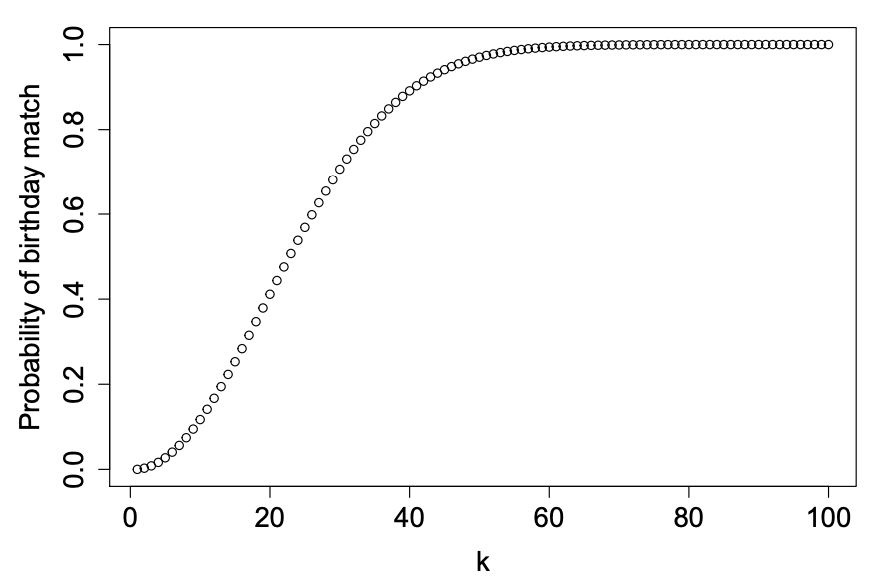
\includegraphics[scale=0.6]{birthday_problem.png}
  \centering
  \caption{Plot probability for increasing k}
\end{figure}  

%----------------------------------------------------
\subsection{Combination}
The cases where order doesn't matter are known as combinations.

\begin{theorem}[Unordered without replacement]
  In the case of sampling \(k\) balls without replacement from an urn of \(n\) balls where order does not matters, we can think of it as drawing \(k\) balls at once, so write the sample space as
  \[\Omega=\{s\in S:|s|=k\}\]
  Then \[|\Omega|=\frac{(n)_k}{k!}=\frac{n!}{k!(n-k)!}=:\binom{n}{k}\]
  where \(\binom{n}{k}\) the \emph{binomial coefficient} or ``\(n\) choose \(k\)'' is defined.
\end{theorem}
\begin{proof}
  We can choose \(k\) from \(n\) without replacement with order first (\((n)_k\)), then divides by the number of ways to order the \(k\) balls (\(k!\)) to eliminate the overcounting.
\end{proof}

We should also note that we are dealing with \(0\leq k\leq n\) here. It gets weird when this is not satisfied.

\begin{exercise}
  Prove the following formulae with counting arguments (story proof):
  \begin{enumerate}
    \item (Sum of coefficients)\[\sum_{k=0}^n\binom{n}{k}=2^n\]
    \item (Binomial theorem) \[(x+y)^n=\sum_{k=0}^n \binom{n}{k}x^ky^{n-k}\]
    \item (Vandermonde's identity) For \(k,m,n\in\N\cup\{0\},k
    \leq m+n\), we have \[\binom{m+n}{k}=\sum_{i=0}^k\binom{m}{i}\binom{n}{k-i}\]
  \end{enumerate}
\end{exercise}
\begin{proof}
  \begin{enumerate}
    \item LHS count the number of all subsets in a set with \(n\) elements, which is equal to RHS as each element can be either in or not in a subset. Differentiate this result will give some other useful identities.
    \item LHS yields sum of \(2^n\) products of the form \(x^ky^{n-k}\) for some \(0\leq k\leq n\). For each \(k\), we need \(x\) appears in exactly \(k\) positions of a \(n\)-string of \(x,y\), so \(\binom{n}{k}\) ways of doing so.
    \item Choosing \(k\) from a set of \(m+n\) is equivalent to choosing \(i\) people from the set of \(m\) and \(k-i\) people from the set of \(n\) for all \(0\leq i\leq k\).
  \end{enumerate}
\end{proof}

\begin{theorem}[Unordered with replacement]
  In the case of sampling \(k\) balls with replacement from an urn of \(n\) balls where order does not matters, we can write the sample space as
  \[\Omega=\{\omega:\omega \text{ is a k-element multiset with elements from } \{1,...,n\}\}\]
  where multiset is a set that allows repeated elements.
  We have \(|\Omega|=\binom{n+k-1}{k}\). Note that we can have \(k>n\) as we are sampling with replacement.
\end{theorem}
\begin{proof}
  This proof is commonly known as the ``stars and bars'' argument. Consider drawing \(n\) distinguishable boxes (labeled balls) using \(n+1\) ``bars''. Distributed among these boxes (between bars) we have \(k\) indistinguishable ``stars'' (number of times the balls get picked). Fixing the outer 2 bars, we have \(n-1\) bars and \(k\) stars to arrange. We can choose either stars or bars first and fill in the rest, giving
  \[|\Omega|=\binom{n+k-1}{k}=\binom{n+k-1}{n-1}\]
\end{proof}

\setlength{\extrarowheight}{5pt}
\begin{table}[ht]
  \centering
  \begin{tabular}{ c | c | c }
    & Ordered & Unordered \\
    \hline
    With replacement & \(n^k\) & \(\binom{n+k-1}{k}\) \\ [5pt] 
    \hline
    Without replacement & \((n)_k\) & \(\binom{n}{k}\) \\[5pt]
  \end{tabular}
  \caption{Summary table for counting}
\end{table}

\begin{extension}{Inclusion-exclusion and derangement}
  %EXT derangement
\end{extension}

%=========================================================
\section{Probability}
\subsection{Probability axioms}
The theory of probability is constructed axiomatically first by Kolmogorov in 1933.

We first introduce the notion of event space \(\cal{F}\), consisting of subsets of \(\Omega\), which is required to be a \(\sigma\)-algebra.
\begin{definition}[Algebra and \(\sigma\)-algebra]
  A collection of subsets of \(\Omega\) denoted by \(\cal{F}\) is called an algebra (or field) on \(\Omega\) if
  \begin{enumerate}
    \item \(\emptyset\in\cal{F}\)
    \item \(\cal{F}\) is closed under complements, \(A\in\cal{F}\implies A^\complement\in\cal{F}\)
    \item \(\cal{F}\) is closed under pairwise union, \(A_1,A_2\in\cal{F}\implies A_1\cup A_2\in\cal{F}\)
  \end{enumerate}
  It is a \(\sigma\)-algebra (or \(\sigma\)-field) on \(\Omega\) if \(\cal{F}\) is also closed under \emph{countable} union.
\end{definition}
\begin{remark}
  Note we also have the following properties
  \begin{enumerate}
    \item Any algebra is closed under finite union and intersection by repeat application of condition 3 and the fact that \(\cap_iA_i=(\cup_iA_i^\complement)^\complement\) where each \(A_i^\complement\in\cal{F}\) by condition 2.
    \item Similarly, any \(\sigma\)-algebra is closed under couuntably infinite union and intersection.
    \item Any algebra contains \(\Omega=\emptyset^\complement\).
  \end{enumerate}
\end{remark}
\begin{example}
  Consider any sample space \(\Omega\). Then,
  \begin{enumerate}
    \item \(\cal{F}=\{\emptyset,\Omega\}\) is the trivial \(\sigma\)-field
    \item \(\cal{F}=\cal{P}(\Omega)\) is the total/power \(\sigma\)-field
    \item \(\cal{F}=\{\emptyset,\Omega,A,A^\complement\}\) is the smallest \(\sigma\)-field containing \(A\subseteq\Omega\)
  \end{enumerate}
\end{example}
In probability we typically define a probability measure (defined below) first on an algebra, then extend it to a \(\sigma\)-algebra. The details would be studied in measure theory. For now, we can assume all \(\cal{F}\) is a \(\sigma\)-algebra.

\begin{definition}[Probability measure]
  A mapping \(P:\cal{F}\to\R\) is called a probability measure on \((\Omega,\cal{F})\) if it satisfies:
  \begin{enumerate}
    \item \(P(A)\geq 0\) for all events \(A\in\cal{F}\)
    \item \(P(\Omega)=1\)
    \item For any countable sequence of disjoint events \(A_i\in\cal{F},\,i\in\cal{I}\), we have \[P\left(\bigcup_{i\in\cal{I}}A_i\right)=\sum_{i\in\cal{I}}P(A_i)\]
    Here disjoint means \(A_i\cap A_j =\emptyset\) for all \(i,j\in\cal{I}\).
  \end{enumerate}  
\end{definition}
These 3 conditions are known as the \emph{Kolmogorov axioms}, named after Russian mathematician Andrey Kolmogorov, who set the foundation for probability theory in 1933.

\begin{definition}[Probability space]
  We define a probability space as the triplet \((\Omega,\cal{F},P)\), where \(\Omega\) is a set (sample space), \(\cal{F}\) is a \(\sigma\)-algebra (event space), and \(P\) a probability measure on \((\Omega,\cal{F})\).
\end{definition}

\begin{proposition}[Properties of probability measure]
  Consider a probability space \((\Omega,\cal{F},P)\). For any \(A,B\in\cal{F}\), we have
  \begin{enumerate}
    \item \(P(A^\complement)=1-P(A)\)
    \item If \(A\subseteq B\) then \(P(A)\leq P(B)\)
    \item \(P(A\cup B)=P(A)+P(B)-P(A\cap B)\)
  \end{enumerate}
\end{proposition}

\begin{proof}
  \begin{enumerate}
    \item Since \(A,A^\complement\) are disjoint, we have \(1=P(\Omega)=P(A\cup A^\complement)=P(A)+P(A^\complement)\).
    \item Express \(B\) in disjoint unions: \(B=(B\cap A)\cup(B\cap A^c)\). Since \(A\subseteq B\), \(B\cap A =A\). So \(P(B)= P(A)+P(B\cap A^c)\geq P(A)\) as probability measure is non-negative.
    \item Express \(A,B\) as disjoint subset as shown above, and also note \(A\cup B= (A\cap B)\cup(A^c\cap B)\cup(A\cap B^c)\). Use axiom 3 and rearrange gives result.
  \end{enumerate}

\end{proof}

\begin{exercise}[Poisson]
  Let \(\Omega=\N, \cal{F}=\cal{P}(\Omega), P:\cal{F}\to\R\) with \(P(A)=\sum_{x\in A}\frac{e^{-\lambda}\lambda^x}{x!}\). Prove that \((\Omega,\cal{F},P)\) forms a probability space.
\end{exercise}
\begin{solution}
  We know that the power set is a \(\sigma\)-algebra, so we only need to show the probability measure satisfies the three Kolmogorov axioms:

  \subproof{}
  Note that
  \(P(\Omega)=\sum_{x\in\Omega}\frac{e^{-\lambda}\lambda^x}{x!}\sum_{x=0}^{\infty}\frac{e^{-\lambda}\lambda^x}{x!}=e^{-\lambda}\sum_{x=0}^{\infty}\frac{\lambda^x}{x!}=e^{-\lambda}e^{\lambda}=1\)
  \subproof{}
  For all \(A\in\cal{F}\), \(P(A)\geq 0\) as \(\lambda >0, e^{-\lambda}>0, \text{ and }  x! >0 \)
  \subproof{}
  Let \(A_i\in\cal{F}\) be a series of countable disjoint events. Then
  \[P\left(\bigcup_{i=1}^\infty A_i\right)=\sum_{x\in A_i}\sum_{i=1}^\infty\frac{e^{-\lambda}\lambda^x}{x!}=\sum_{i=1}^\infty\sum_{x\in A_i}\frac{e^{-\lambda}\lambda^x}{x!}=\sum_{i=1}^\infty P(A_i)\]
  by interchanging order of summation, as covered in analysis.
\end{solution}

%----------------------------------------------------
\subsection{Conditional probability}
\begin{definition}[Conditional probability]
  Consider a probability space \((\Omega,\cal{F},P)\). Then the conditional probability of \(A\) given \(B\) is defined as
  \[P(A|B)=\frac{P(A\cap B)}{P(B)}\]
\end{definition}

\begin{theorem}
  Given a probability space \((\Omega,\cal{F},P)\). Let \(B\in\cal{F}\) with \(P(B)>0\) and define \(Q:\cal{F}\to\R\) by \(Q(A)=P(A|B)\) Then \((\Omega,\cal{F},Q)\) is a probability space.
\end{theorem}
\begin{proof}
  \subproof{}
  Clearly
  \[Q(\Omega)=\frac{P(\Omega\cap B)}{P(B)}=\frac{P(B)}{P(B)}=1\]
  \subproof{}
  \(P\) is probability measure so non-negative. Hence \(Q(A)=\frac{P(A\cap B)}{P(B)}\geq 0\).
  \subproof{}
  For any countable series of disjoint events \(A_i,i\in\cal{I}\), we have 
  \[Q\left(\bigcup_{i\in\cal{I}}A_i\right)= \frac{(P(\cup_{i\in\cal{I}}A_i)\cap B)}{P(B)} = \frac{P(\cup_{i\in\cal{I}}(A_i \cap B))}{P(B)}=\frac{\sum_{i\in\cal{I}}P(A_i\cap B)}{P(B)}\] 
\end{proof}

We now have \(P(A\cap B)=P(A|B)P(B)\) and \(P(B\cap A)=P(B|A)P(A)\). Since \(P(A\cap B)=P(B\cap A)\), we have 
\begin{theorem}[Bayes' theorem]
  Let \(A,B\in\cal{F}\) such that \(P(A)>0,P(B)>0\), then
  \[P(A|B)=\frac{P(B|A)P(A)}{P(B)}\]
\end{theorem}

If we extend the first part of the argument above, treating \(B\) as \(B\cap C\). we have \(P(A\cap B\cap C)=P(A|B\cap C)P(B|C)P(C)\). This works inductively, giving

\begin{theorem}[Multiplication rule]
  For any \(A_i,i\in\N\) with \(P(A_2\cap...\cap A_n)>0\), we have
  \[P(A_1\cap ... \cap A_n)=P(A_1|A_2\cap...\cap A_n)P(A_2|A_3\cap...\cap A_n)...P(A_{n-1}|A_n)P(A_n)\]
\end{theorem}

\begin{definition}[Partition]
  A partition of a sample space \(\Omega\) is a collection \(\{B_i:i\in\cal{I}\}\) of disjoint such that \(\Omega=\cup_{i\in\cal{I}}B_i\).
\end{definition}

\begin{theorem}[Law of total probability]
  If \(\{B_i:i\in\cal{I}\}\) is a partition and \(P(B_i)>0\), then
  \[P(A)=\sum_{i\in\cal{I}}P(A\cap B_i)=\sum_{i\in\cal{I}}P(A|B_i)P(B_i)\]
\end{theorem}
\begin{proof}
  We have \(A=A\cap\Omega=A\cap\bigcup_{i\in\cal{I}}B_i\). Use distributitve law, we have \(A=\bigcup_{i\in\cal{I}}(A\cap B_i)\). Then since \(B_i\) are disjoints, by the 3rd Kolmogorov axiom (countable additivity), we have \(A=\sum_{i\in\cal{I}}P(A\cap B_i)\).

  For the 2nd equation, simply apply the multiplication rule.
\end{proof}

The law of total probability provides a useful way to find \(P(A)\) (in Bayes', for instance) which could otherwise be quite hard to find.

It is sometimes useful to have one extra condition, the following can be easily proved using the definition of conditional probability and law of total probability rule.
\begin{proposition}[Additional conditioning]
  Consider events \(A,B,E\in\cal{F}\) and \(\{B_i,i\in\cal{I}\}\) a partition of \(\Omega\).
  \begin{itemize}
    \item (Bayes') if \(P(A\cap E),P(B\cap E)>0\), then \[P(A|B\cap E)=\frac{P(B|A\cap E)P(A|E)}{P(B|E)}\]
    \item (total probability) if \(P(E)>0\) and \(P(B_i\cap E)>0\) for all \(B_i\), then \[P(A|E)=\sum_i\frac{P(A\cap B_i\cap E)}{P(E)}=\sum_i P(A|B_i\cap E)P(B_i|E)\]
  \end{itemize}
\end{proposition}

\begin{exercise}[Disease test]
  Consider a ‘mammography test on a population with a 1 \% prevalence of breast cancer. The test is positive for around 90\% of women with cancer, but it is also positive for around 10\% of women without cancer’.  
  What is the probability that a woman whose mammography test is positive has breast cancer?
\end{exercise}
\begin{solution}
  Define the events: B := breast cancer present; T := test is positive. We know that \(P(B)=0.01\) and \(P(T|B)=0.1\) so \(P(T|B^c)=0.9, P(B^c)=0.99\). 

  By Bayes' rule and law of total probability, we have 
  \[P(B|T)=\frac{P(T|B)P(B)}{P(T|B)P(B)+P(T|B^c)P(B^c)}=\frac{0.009}{0.108}\approx 8\%\]
\end{solution}

\begin{exercise}[Monty Hall]
  A contestant selects one of three doors: behind one of the doors there is a car, and others are goats. After the contestant selects a door, Monty Hall opens one of the remaining doors, and reveals that there is no prize behind it. The host then asks the contestant whether they want to SWITCH their choice to the other unopened door, or STICK to their original choice. Which one should the contestant choose?
\end{exercise}
\begin{solution}
  WLOG suppose the contestant chose door 1. Denote partition \(\{C_1,C_2,C_3\}\) the events that the car is behind door \(i\). Denote \(H_2\) as Mr Hall reveals door 2. Then we want to compare the probability STICK:\(P(C_1|H_2)\) and SWITCH:\(P(C_3|H_2)\).

  Note \(P(C_i)=1/3\) and \(P(H_2|C_1)=1/2, P(H_2|C_2)=0, P(H_2|C_3)=1\), so by total probability, \(P(H_2)=1/2\). Then, by Bayes, we have \[P(C_1|H_2)=\frac{P(H_2|C_1)P(C_1)}{P(H_2)}=\frac{1}{3} \text{ and } P(C_3|H_2)=\frac{P(H_2|C_3)P(C_3)}{P(H_2)}=\frac{2}{3}\] Hence the contestant should SWITCH.
\end{solution}
%----------------------------------------------------
\subsection{Independence}
\begin{definition}[Independence (pairwise)]
  Two events \(A,B\) are independent if \(P(A\cap B)=P(A)P(B)\).
\end{definition}

\begin{proposition}
  If \(A,B\) are independent, then so are \(A,B^c\); \(A^c,B\); \(A^c,B^c\).
\end{proposition}
\begin{proof}
  We just prove it for \(A,B^c\), the others are largely similar.
  By law of total probability,
  \[P(A)=P(A\cap B)+P(A\cap B^c)=P(A\cap B)+P(A\cap B^c)\]
  Hence using \(A,B\) independent, we have 
  \[P(A)P(B^c)=P(A)(1-P(B))=P(A\cap B)+P(A\cap B^c)-P(A\cap B)=P(A\cap B^c)\]
\end{proof}

\begin{definition}[Independence (general)]
  We say events \(A_1,...,A_n\) are independent if for every subcollection of events \(\{i_1,i_2,...,i_k\}\subseteq\{1,...,n\}\), we have 
  \[P(A_{i_1}\cap...\cap A_{i_k})=P(A_{i_1})...P(A_{i_k})\]

  For infinite collection of events, we say they are independent if each finite subcollection is independent.
\end{definition}

Pairwise independence \((A_i,A_j)\) is NOT sufficient to conclude general independence.
\begin{example}
  Roll a fair 6-sided dice twice. Let \(A_1=\) first roll is odd, \(A_2=\) second roll is odd, \(A_3=\) sum of two rolls is odd. Then \(A_1,A_2,A_3\) are pairwise independent, but \(P(A_1\cap A_2\cap A_3)=0\neq P(A_1)P(A_2)P(A_3)\) 
\end{example}

\begin{definition}[Conditional independence]
  Consider \(A,B,C\in\cal{F}\) with \(P(C)>0\), we say \(A,B\) are conditionally independent given \(C\) if
  \[P(A\cap B|C)=P(A|C)P(B|C)\]
\end{definition}
\begin{remark}
  If \(P(B\cap C)>0\) also, then the above definition is equivalent to
  \[P(A|B\cap C)=P(A|C)\]
  because 
  \[P(A|B\cap C)=\frac{P(A\cap B\cap C)}{P(B\cap C)}=\frac{P(A\cap B|C)P(C)}{P(B\cap C)}=\frac{P(A\cap B|C)}{P(B)}=P(A|C)\]
\end{remark}

\begin{extension}{Gambler's ruin}
  %EXT Gambler's ruin Hwang
\end{extension}

%----------------------------------------------------
\subsection{Continuity}
\begin{definition}[Increasing set]
  A sequence of sets \((A_i)_{i=1}^\infty\) increases to \(A\) if \(A_1\subseteq A_2\subseteq...\) and \(\bigcup_{i=1}^\infty A_i=A\). We denote this as \((A_i)\uparrow A\). 
  
  Similarly for decreasing, \((A_i)\downarrow A\) if \(A_1\supseteq A_2\supseteq...\) and \(\bigcap_{i=1}^\infty A_i=A\).
\end{definition}
Note that \(A_i \uparrow A\) if and only if \(A_i^c\downarrow A^c\).

\begin{lemma}
  Any countable union can be written as a countable union of disjoint subsets.  
\end{lemma}
\begin{proof}
  Given an countable index set \(\cal{I}\) and \(A_i\in\cal{F}\), we define \(D_1=A_1,D_2=A_2\backslash A_1, D_3=A_3\backslash (A_1\cup A_2),...\)
  We claim that \(\{D_i\}\) (which is disjoint by construction) satisfies \(\cup_{i\in\cal{I}}A_i=\cup_{i\in\cal{I}}D_i\).

  \subproof{}
  Suppose \(\omega\in\cup_{i\in\cal{I}}A_i\). Then \(\omega\in A_i\) for at least one \(i\). Let \(I\) be the smallest index \(i\) such that \(\omega\in A_i\). Then \(\omega\notin A_i\) for all \(i<I\). Hence \(\omega\in D_I\) and thus \(\omega\in\cup_{i\in\cal{I}}D_i\) also.
  \subproof{}
  Suppose \(\omega\in\cup_{i\in\cal{I}}D_i\). Then \(\omega\in D_I\) for some \(I\in\cal{I}\), but then \(\omega\in A_I\), and thus \(\omega\in\cup_{i\in\cal{I}}A_i\) also.
  
  They are subsets of each other and so are equal. Note \(n\) does not have to be finite in the argument above.
\end{proof}

\begin{theorem}[Continuity of probability measure]
  If \(A_i\in\cal{F}\) and \(A_i\) increases/decreases to \(A\), then \[\lim_{i\to\infty}P(A_i)=P(\lim_{i\to\infty}A_i)=P(A)\]
\end{theorem}
\begin{proof}
  Suppose \(A_i\uparrow A\). Using lemma above, we write \(A=\cup_{i=1}^\infty A_i=\cup_{i=1}^\infty D_i\) as defined (so \(D_i\) disjoint). Since probability measure is closed under countable unions, we have
  \begin{align*}
    P(A)&=\sum_1^\infty P(D_i)=\lim_{n\to\infty}\sum_i^n P(D_i)\\ &=\lim_{n\to\infty} P(\cup_{i=1}^\infty D_i)=\lim_{n\to\infty} P(\cup_{i=1}^\infty A_i)=\lim_{n\to\infty} P(A_n) 
  \end{align*}

  Suppose \(A_i\downarrow A\). Then \(A_i^c\uparrow A^c\). By above, \(P(A^c)=\lim_{n\to\infty}P(A_i^c)\). We are done using the first probability measure axiom.
\end{proof}

\begin{theorem}[Product rule]
  If \(A_i\) is a countable set of independent events, then
  \[P\left(\bigcap_{i=1}^\infty A_i\right)=\prod_{i=1}^\infty P(A_i)\]
\end{theorem}
\begin{proof}
  Let \(B_n:=\cap_{i=1}^n A_i\). Then \(B_n\downarrow B:=\cap_{i=1}^\infty A_i\). By continuity of probability measure and multiplication principle,
  \[P(B)=\lim_{n\to\infty} P(B_n)=\lim_{n\to\infty}P(\cap_{i=1}^n A_i)=\lim_{n\to\infty}\prod_{i=1}^n P(A_i)=\prod_{i=1}^\infty P(A_i)\]
\end{proof}

%=========================================================
\section{Univariate Random Variables}
\subsection{Random variables}
\begin{definition}[Image and pre-image]
  For a function \(f:X\to Y\) and \(A\subseteq X,B\subseteq Y\), we define \(f_*(A)=\{f(x):x\in A\}\) the image of \(A\) and \(f^*(B)=\{x\in X:f(x)\in B\}\) the pre-image of \(B\).
\end{definition}
If the subset only has 1 element, then it is common to omit the curly braces in writing.

\begin{definition}[Random variables]
  A random variable on the probability space \((\Omega,\cal{F},P)\) is the mapping \(X:\Omega\to\R\) such that for all \(x\in\R\),
  \[X^*(\lointerval{-\infty,x})=\{\omega\in\Omega:X(\omega)\leq x\}\in\cal{F}\]
  The random variable is discrete if the image is countable. Otherwise it's continuous.

  The value \(X(\omega)\) is called the \emph{realisation} of \(X\) at the sample point \(\omega\).
\end{definition}
This definition is rather measure-theoretic. It is sufficient for now to just think of it as a (deterministic) function that assigns a real number to a experimental outcome (e.g. 1 for Head and -1 for Tail in coin toss). The randomness stems from the sample point.

\begin{definition}[Probability mass function]
  The probability mass function (p.m.f.) of a discrete random variable \(X\) is the function \(p_X:\R\to[0,1]\) given by 
  \[p_X(x)=P(X^*(x))\]
\end{definition}

\begin{theorem}
  Let \(\cal{I}\) be a countable index set. Let \(S=\{s_i:i\in\cal{I},s_i\in\R\}\) and \(\Pi=\{\pi_i:i\in\cal{I},\pi_i\in\R\}\), where \(\pi_i\geq 0\) and \(\sum_i \pi_i =1\). 
  
  Then there exists a probability space \((\Omega,\cal{F},P)\) and a discrete random variable \(X\) on the space such that \(p_X(s_i)=\pi_i\) for all \(i\in\cal{I}\) and \(p_X(s)=0\) if \(s\notin S\).
\end{theorem}
\begin{proof}
  Take \(\Omega=S,\cal{F}=\cal{P}(\Omega)\), and \(P\) such that for all \(A\in\cal{F}\),
  \[P(A)=\sum_{i:s_i\in A}\pi_i\]
  Then the d.r.v. on the space, \(X:\Omega\to\R\), is simply \(X(\omega)=\omega\) for all \(\omega\in\Omega\).
\end{proof}
This theorem is useful as it allows us to study discrete random variables without worrying too much about whether the corresponding probability space exists.

\begin{definition}[Cumulative distribution function]
  The cumulative distribution function (c.d.f.) of a random variable \(X\) is the mapping \(F_X:\R\to[0,1]\) given by 
  \[F_X(x)=P(\{\omega\in\Omega:X(\omega)\leq x\})=P(X^*(\lointerval{-\infty,x}))=:P(X\leq x)\] 
\end{definition}

\begin{proposition}[Properties of c.d.f.]
  \begin{enumerate}
    \item \(F_X\) is increasing (not strictly): \(F_X(x)\leq F_X(y), \forall x\leq y\)
    \item \(F_X\) is right-continuous: if \((x_n)\) is a decreasing sequence that converges to \(x\), i.e. \(x_n\downarrow x\), then \(F_X(x_n)\to F_X(x)\) as \(n\to\infty\)
    \item \(\lim_{x\to-\infty}F_X(x)=0,\lim_{x\to\infty}F_X(x)=1\)
  \end{enumerate}
\end{proposition}
\begin{proof}
  \subproof{}
  Follows immediately from monotonicity of probability measure.
  \subproof{}
  Since we have \(x_1\geq...\geq x_n\geq...\geq x\) and \(\lim_{n\to\infty}x_n=x\), can define
  \[E_n:=\{\omega:X(\omega)\leq x_n\}\downarrow \bigcap_{n=1}^\infty E_n=\{\omega:X(\omega)\leq x\}=:E\]
  Then \(P(E_n)=F_X(x_n),P(E)=F_X(x)\). By continuity, \(\lim_{n\to\infty}P(E_n)=P(E)\). Done.
  \subproof{}
  Define \(E_n\) as above for arbitrary \((x_n)\). Then \(E_n\downarrow\emptyset\) as \(x_n\downarrow -\infty\) and \(E_n\uparrow\Omega\) as \(x_n\uparrow\infty\). By continuity, \(F_X(x_n)=P(E_n)\to P(\emptyset)=0,F_X(x_n)=P(E_n)\to P(\Omega)=1\). 
\end{proof}
In fact, one can show that for any function \(F\) satisfying the above properties, there exists a probability space and a random variable on that space which has \(F\) as its c.d.f..

\begin{remark}
  Note that \(F_X\) is in general not left-continuous. Consider a sequence \(x_n\uparrow x\). Then define \(E_n\) in a similar way gives 
  \[E_n\uparrow \bigcup_{n=1}^\infty E_n = \{\omega:X(\omega)<x\}=:E\] 
  Note inequality inside \(E\) is strict, namely, \(E=\{\omega:X(\omega)\leq x\}\cup\{\omega:X(\omega)=x\}\). Hence \(P(E)=\lim_{n\to\infty}E_n\) if and only if \(P(\{\omega:X(\omega)=x\})=0\), using continutiy.
\end{remark}

\begin{theorem}
  For \(a<b\), we have \(P(a<x\leq b)=F_X(b)-F_X(a)\)
\end{theorem}
\begin{proof}
  Note that \[\{\omega:X(\omega)\leq b\}=\{\omega:X(\omega)\leq a\}\cup \{\omega:a<X(\omega)\leq b\}\]
  Since they are disjoint, use axiom 3 and rearrange gives required result.
\end{proof}

\begin{definition}[Probability density function]
  The probability density function (or density) of a continous random variable \(X\) is the function \(f_x:\R\to\R\) such that for all \(x\in\R\),
  \[F_X(x)=P(X\leq x)=\int_{-\infty}^{x}f_X(u)\,du\]
\end{definition}

\begin{theorem}
  For a continuous random variable \(X\) with density \(f_X\), we have, for all \(x\in\R\)
  \[P(X=x)=0\]
  and for all \(a\leq b, a,b\in\R\)
  \[P(a\leq x\leq b)=\int_{a}^{b}f_X(u)\,du\]
\end{theorem}
\begin{proof}
  Consider arbitrary \(x\in\R\) and \(x_n\uparrow x\). Define
  \[E_n:=\{\omega:x_n<X(\omega)\leq x\} \downarrow \{\omega:X(\omega)=x\}=:E\]
  Then, using continuity, we have \(P(E_n)\to P(E)\) as \(n\to\infty\). Hence 
  \[
    P(X=x) = \lim_{n\to\infty}P(E_n) = \lim_{n\to\infty}(F_X(x)-F_X(x_n)) = \lim_{n\to\infty}\int_{x_n}^{x}f_X(u)\,du=0
  \]
  It follows that for \(a<b\), we have
  \[P(a\leq x\leq b)=P(a<x\leq b)=\int_{a}^{b}f_X(u)\,du\]
\end{proof}

%----------------------------------------------------
\subsection{Common discrete distribution}
It is assumed for distributions below that \(P(X=x)=0\) if \(x\notin X_*\), the image of \(X\). It is left as exercise to verify each p.m.f. is valide, i.e. \(P(X=x)>0,\:\forall x\) and \(\sum_xP(X=x)=1\).
\begin{definition}[Bernoulli distribution]
  A discrete random variable \(X\) follows a Bernoulli distribution with parameter \(p\in(0,1)\), i.e. \(X\sim \rm{Bern}(p)\), if \(X_*=\{0,1\}\) and
  \begin{equation*}
    P(X=x)=\begin{cases}
      p & \text{ if } x=1 \\
      1-p & \text{ if } x=0\\
    \end{cases}
  \end{equation*}
\end{definition}
For any event, there is a natural way to associate a Bernoulli random variable with it. 
\begin{definition}[Indicator variable]
  Consider an event \(A\in\cal{F}\). We define the indicator variable of \(A\) by
  \[\mathbb{I}_A(\omega)=\begin{cases}
    1 & \text{ if } \omega\in A\\
    0 & \text{ if } \omega\notin A\\
  \end{cases}\]
  Hence \(\mathbb{I}_A\sim \rm{Bern}(P(A))\).
\end{definition}
An experiment with two outcomes (success or failure) is called a \emph{Bernoulli trial}. Hence a Bernoulli variable can be think of an indicator of success with success probability \(p\).

\begin{definition}[Binomial distribution]
  A discrete random variable \(X\) follows a binomial distribution with parameters \(n\in\N\) and \(p\in(0,1)\), i.e. \(X\sim \rm{Bin}(n,p)\), if \(X_*=\{0,1,...,n\}\) and
  \[P(X=x)=\binom{n}{x}p^x(1-p)^{n-x}\]
\end{definition}
Binomial distribution models the number of success in a sequence of \(n\in\N\) independent and identical Bernoulli trials with success probability \(p\). This is clear: the probability of \(x\) success occuring in a sequence of \(n\) trials is \(p^x(1-p)^{n-x}\), and there are \(\binom{n}{x}\) possible \(n\) strings with \(x\) successes. 

\begin{definition}[Hypergeometric distribution]
  A discrete random variable \(X\) follows a hypergeometric distribution with parameters \(N\in\N\cup\{0\}\), \(K,n\in\{0,1,...,N\}\), i.e. \(X\sim \rm{HGeo}(N,K,n)\), if \(X_*=\{0,1,...,\min(n,k)\}\) and 
  \[P(X=x)=\frac{\binom{K}{x}\binom{N-K}{n-x}}{\binom{N}{n}}=\frac{\binom{n}{x}\binom{N-n}{K-x}}{\binom{N}{K}}\]
\end{definition}
Consider an urn with \(N\) balls, of which \(K\) are white and the rest are black. Hypergeometric distribution models the number of white balls in a draw of \(n\) balls without replacement. We require each balls to be distinguishable, although order doesn't matter.

\vspace{5pt}The 1st formula is true because we need to choose \(x\) white balls from the \(K\) white balls available and \(n-x\) from the rest. The denominator is the total way of choosing a set of \(n\) balls. The 2nd formula is equivalent because the scenario can be modelled as drawing out \(n\) from \(N\) black balls first, then painting \(x\) of them white outside the urn and \(K-x\) inside. The denominator is the total way of painting \(K\) whites.

\vspace{5pt}We may use the Vandermonde's identity discussed earlier to show it is a valide p.m.f.
\begin{definition}[Uniform distribution]
  Let \(C\) be a finite non-empty set of numbers. A discrete random variable \(X\) follows a discrete uniform distribution on \(C\), i.e. \(X\sim \rm{DUnif}(C)\), if \(X_*=C\) and
  \[P(X=x)=\frac{1}{|C|}\]
\end{definition}
This simply represents an experiment where each outcomes is equally likely.

\begin{definition}[Poisson distribution]
  A discrete random variable \(X\) follows a Poisson distribution with parameter \(\lambda>0\), i.e. \(X\sim \rm{Po}(\lambda)\), if \(X_*=\N\cup\{0\}\) and
  \[P(X=x)=\frac{e^{-\lambda}\lambda^x}{x!}\]
\end{definition}
Poisson distribution is extremely useful, widely used for counting the occurence of some events over a certain time period.

\begin{definition}[Geometric distribution]
  A discrete random variable \(X\) follows a geometric distribution with parameter \(p\in(0,1)\), i.e. \(X\sim \rm{Geo}(p)\), if \(X_*=\N\) and
  \[P(X=x)=(1-p)^{x-1}p\]
\end{definition}
Geometric distribution models the number of independent Bernoulli trials to obtain the first success when repeating an experiment with success probability \(p\).

\begin{definition}[Negative binomial distribution]
  A discrete random variable \(X\) follows a negative binomial distribution with parameter \(r\in\N\) and \(p\in(0,1)\), i.e. \(X\sim \rm{NBin}(p)\), if \(X_*=\N\cup\{0\}\) and
  \[P(X=x)=\binom{x+r-1}{r-1}p^r(1-p)^x\]
\end{definition}
The negative binomial distribution is some sort of extension to the geometric distribution. It counts the number of failures in a sequence of independent Bernoulli trials with success probability \(p\) before \(r\) successes have occured.

\vspace{5pt}To see this, consider strings of \(0,1\) for failure/success. Each string with \(r\) 1s and \(x\) 0s occurs with probability \(p^r(1-p)^x\). How many such strings are there? We stop when reaching \(r\)th success so last digit must be 1. Hence we just need to choose the reaming \(r-1\) 1s among \(x+r-1\) positions, giving \(\binom{x+r-1}{r-1}\) possibilities.

\vspace{5pt}To prove that it is a valid p.m.f., we may use the generalised binomial theorem.
\begin{theorem}[Generalised binomial theorem]
  For \(a\in\C\), we have
  \[(1+x)^a=\sum_{k=0}^\infty\frac{a(a-1)...(a-k+1)}{k!}x^k\]
\end{theorem}
\begin{lemma}
  For \(x\in\N\cup\{0\},r\in\N\), we have
  \[\binom{x+r-1}{r-1}=(-1)^x\binom{r}{x}\]
\end{lemma}
The proof is simply algebraic manipulation.

%----------------------------------------------------
\subsection{Common continuous distribution}

It is assumed for distributions below that \(f(x)=0\) if \(x\notin X_*\). Section for interest only.
\begin{definition}[Continuous uniform distribution]
  A continuous random distribution \(X\) follows a uniform distribution on an interval \((a,b)\), i.e. \(X\sim \rm{U} (a,b)\), if \(X_*=(a,b)\) and its density is 
  \[f(x)=\frac{1}{b-a}\]
\end{definition}

\begin{definition}[Exponential distribution]
  A continuous random distribution \(X\) follows an exponential distribution with parameter \(\lambda >0\), i.e. \(X\sim \rm{Exp}(a,b)\), if \(X_*=\R_{>0}\) and its density is 
  \[f(x)=\lambda e^{-\lambda x}\]
\end{definition}

\begin{definition}[Gamma distribution]
  A continuous random distribution \(X\) follows a Gamma distribution with shape parameter \(\alpha >0\) and rate parameter \(\beta >0\), i.e. \(X\sim \rm{Gamma}(\alpha,\beta)\), if \(X_*=\R_{>0}\) and its density is 
  \[f(x)=\frac{\beta^\alpha}{\Gamma(\alpha)}x^{\alpha-1}e^{-\beta x}\]
  where \(\Gamma(t)\) the gamma function is an extension to factorial given by
  \[\Gamma(t)=\int_{0}^{\infty}x^{t-1}e^{-x}\,dx\] 
\end{definition}

\begin{definition}[Chi-squared distribution]
  A continuous random distribution \(X\) follows a chi-squared distribution with degree of freedom \(n\in\N\), i.e. \(X\sim \chi^2_n\), if and only if \(X\sim \rm{Gamma}(n/2,1/2)\).
\end{definition}

\begin{definition}[Beta distribution]
  A continuous random distribution \(X\) follows a beta distribution with parameters \(\alpha,\beta >0\), i.e. \(X\sim \rm{Beta}(\alpha,\beta)\), if \(X_*=[0,1]\) and its density is 
  \[f(x)=\frac{1}{B(\alpha,\beta)}x^{\alpha-1}(1-x)^{\beta-1}\]
  where \(B(\alpha,\beta)\) the beta function is given by
  \[B(\alpha,\beta)=\int_{0}^{1}x^{\alpha-1}(1-x)^{\beta-1}\,dx=\frac{\Gamma(\alpha)\Gamma{\beta}}{\Gamma{\alpha+\beta}}\]
\end{definition}

\begin{definition}[Normal/Gaussian distribution]
  A continuous random distribution \(X\) follows a normal distribution with mean \(\mu\in\R\) and standard deviation \(\sigma>0\), i.e. \(X\sim \rm{N}(\mu,\sigma^2)\), if \(X_*=\R\) and its density is 
  \[f(x)=\frac{1}{\sigma\sqrt{2\pi}}e^{-\frac{(x-\mu)^2}{2\sigma^2}}\]
  If \(\mu=0,\sigma=1\), then it is called the standard normal distribution, denoted as \(Z\).

  We also denote the cumulative function of the standard normal distribution as \(\Phi\).
\end{definition}

\begin{definition}[Cauchy distribution]
  A continuous random distribution \(X\) follows a Cauchy distribution if \(X_*=\R\) and its density is 
  \[f(x)=\frac{1}{\pi(1+x^2)}\]
\end{definition}
Note that \(Z=X/Y\) follows a Cauchy distribution if \(X,Y\) follows \(\rm{N}(0,1)\).

\begin{definition}[T-distribution]
  A continuous random distribution \(X\) follows a t-distribution with degrees of freedom \(\nu >0\) if \(X_*=\R\) and its density is
  \[f(x)=\frac{\Gamma(\frac{\nu+1}{2})}{\Gamma(\frac{\nu}{2})\sqrt{\nu\pi}}\left(1+\frac{x^2}{\nu}\right)^{-\frac{\nu+1}{2}}\]
\end{definition}

Although most distribution we encounter would be either discrete or continuous, it is important to recognise that these are not the only case. Here is an example.

\begin{example}[Distribution that is neither discrete nor continuous]
  We flip infinitely many times an unfair coin with probability \(p\in(0,1)\) and \(p\neq 0.5\) of getting head. Denote \(X_i=0\) for getting tail on the \(i\)th flip and \(X_i=1\) otherwise. Define also \(Y=0.X_1X_2...\) Recall from analysis that the set of \(Y\) is uncountable using diagonal argument.

  Note that for any \(y=0.x_1x_2...\) in base 2, the following infinite product converge to 0,
  \[P(Y=y)=P(X_1=x_1)P(X_2=x_2)...=0\]
  since \(p\in( 0,1)\). Hence \(Y\) cannot be discrete.

  It can also be show that \(Y\) does not have a density.%EXT
\end{example}
%----------------------------------------------------
\subsection{Transformation}
\begin{theorem}[Discrete transformation]
  Let \(X\) be a discrete random variable and let \(g:X_*\to\R\) be a deterministic function. Then \(Y=g(X)\) is a discrete random variable with pmf given by
  \[p_Y(y)=\sum_{x\in g^*(y)}P(X=x)\]
\end{theorem}
\begin{proof}
  %TODO transformation
\end{proof}

\begin{theorem}[Continuous transformation]
  Let \(X\) be a continuous random variable with density \(f_X\). Let \(g:\R\to\R\) be strictly monotonic, differentiable, with inverse \(g^{-1}\). Then \(Y=g(X)\) has density
  \[f_Y(y)=f_X(g^{-1}(y))\left|\diff{}{y}g^{-1}(y)\right|=f_X(x)\left|\diff{x}{y}\right|\]
\end{theorem}
Note that strict monotonicity of a function implies its invertibility.
\begin{proof}
  %
\end{proof}

\begin{example}[Transformation of normal distribution]
  Let \(Z\sim\rm{N}(0,1)\) and \(X=\sigma Z+\mu\) for \(\sigma,\mu>0\). Compute the p.d.f. of \(X\).

  We first find the c.d.f of \(X\):
  \[P(X\leq x)=P(\sigma Z+\mu \leq x)=P(Z\leq (x-\mu)/\sigma)=\Phi((x-\mu)/\sigma)\]
  
  Differentiate this then gives
  \[P(X=x)=\diff{}{x}P(X\leq x)=\frac{1}{\sigma\sqrt{2\pi}}e^{-\frac{(x-\mu)^2}{2\sigma^2}}\]
  so \(X\sim\rm{N}(\mu,\sigma)\). It follows that any linear transformation of a normal variable is still a normal variable.
\end{example}


%----------------------------------------------------
\subsection{Expectation and variance}
\begin{definition}[Expectation]
  Let \(X\) be a random variable with pmf \(p\)/pdf \(f\), then the expectation of \(X\) is
  \[E(X)=\begin{cases}
    \sum_{x\in X_*}xp(x)&\text{ if \(X\) is discrete}\\ 
    \int_{-\infty}^{\infty}xf(x)\,dx&\text{ if \(X\) is continuous }
  \end{cases}\]
\end{definition}

\begin{proposition}[Algebra of expectation]
  For any random variable \(X\) with finite expectation and constants \(a,b\in\R\), we have
  \[E(aX+b)=aE(X)+b\]
\end{proposition}
\begin{proof}
  %TODO expectation and variance
\end{proof}

\begin{theorem}[Law of the unconscious statistician (LOTUS)]
  Let \(X\) be a random variable with pmf \(p\)/pdf \(f\), and \(g:\R\to\R\) a function, then
  \[E(g(X))=\begin{cases}
    \sum_{x\in X_*}g(x)p(x)&\text{ if \(X\) is discrete}\\ 
    \int_{-\infty}^{\infty}g(x)f(x)\,dx&\text{ if \(X\) is continuous }
  \end{cases}\]
\end{theorem}
The proof is non-trivial, although it may not look like it, hence the name.
\begin{proof}
  %
\end{proof}

\begin{definition}[Variance]
  For a random variable \(X\), its variance is given by
  \[Var(X)=E[(X-E(X))^2]\]
\end{definition}
\begin{theorem}
  For any random variable \(X\) with finite variance, we have 
  \[Var(X)=E(X^2)-E(X)^2\]
\end{theorem}
\begin{proof}
  %
\end{proof}

\begin{proposition}[Algebra of variance]
  For any random variable \(X\) with finite variance and constants \(a,b\in\R\), we have
  \[Var(aX+b)=a^2Var(X)\]
\end{proposition}
\begin{proof}
  %
\end{proof}

%=========================================================
\section{Bivariate Random Variables}
\subsection{Joint random variables}
\begin{definition}[Joint distribution function]
  The joint distribution function of the random vector \((X,Y)\) is the mapping \(F_{X,Y}:\R^2\to[0,1]\) given by (the shorthand)
  \[F_{X,Y}(x,y)=P(X\leq x,Y\leq y)\]
  for any \(x,y\in\R\). Their joint pmf/pdf is then given by 
  \[p_{X,Y}(x,y)=P(X=x,Y=y), \; f_{X,Y}(x,y)=\diffp{}{{x}{y}}F_{X,Y}(x,y)\]
\end{definition}
We will omit the subscript for the bivariate variables below.

\begin{definition}[Marginal distribution]
  The marginal distributiion of \(X\) for \(F(x,y)\) is defined as
  \[F_X(x)=\lim_{y\to\infty}F(x,y)\]
  Its marginal density is then given by 
  \[p_X(x)=\sum_{y}p(x,y),\; f_X(x)=\int_{a}^{b}f(x,y)\,dy\]
  where \(x\in[a,b]\). Likewise for \(Y\).
\end{definition}
We obviously require non-negativity and sum/integrate to unity for above pmf/pdf.

\begin{proposition}
  The following properties hold for joint distribution function \(F_{X,Y}\):
  \begin{itemize}
    \item increasing in each variable
    \item continous from above (the multivariate version of right continuity)
    \item \(\lim_{x\to -\infty,y\to -\infty}F(x,y)=0, \lim_{x\to \infty,y\to \infty}F(x,y)=1\)
    \item Determine their marginal distribution uniquely
  \end{itemize}
\end{proposition}

\begin{definition}[Independence]
  Random variables \(X,Y\) are independent if for all \(x,y\)
  \[P(X\leq x,Y\leq y)=P(X\leq x)P(Y\leq y)\]
  In fact, this is equivalent to
  \[p(x,y)=p_X(x)p_Y(y),\; f(x,y)=f_X(x)f_Y(y)\]
\end{definition}

\begin{theorem}[2d-LOTUS]
  The law of the unconscious statistician applies to the bivariate case too.
  \[E(g(X,Y))=\int_{-\infty}^{\infty}\int_{-\infty}^{\infty}g(x,y)f(x,y)\,dxdy\]
  \[E(g(X,Y))=\sum_x\sum_y g(x,y)P(X=x,Y=y)\]
\end{theorem}

\begin{definition}[Covariance and Correlation]
  For joint random variables \(X,Y\), we define their covariance as
  \[\rm{Cov}(X,Y)=E((X-E(X))(Y-E(Y)))\]
  if the expectation takes a finite value. Their correlation is defined as
  \[\rm{Cor}(X,Y)=\frac{\rm{Cov}(X,Y)}{\sqrt{Var(X)Var(Y)}}\]  
\end{definition}
\begin{theorem}
  For joint random variables \(X,Y\) with finite expectations, we have
  \[\rm{Cov}(X,Y)=E(XY)-E(X)E(Y)\]
\end{theorem}

\subsection{Transformation}
Consider the case of jointly continuous random variables \((X,Y)\) with density \(f\). Let \(u,v:\R^2\to\R\) be deterministic functions, and define random variables
\[U=u(x,y),\; V=v(x,y)\]
We would like to find the joint density of \((U,V)\).

Define the mapping \(T:\R^2\to\R^2\) by 
\[T(x,y)=(u(x,y),v(x,y))\]
which is a bijection from domain \(D\) to some range \(S\). Then we have an inverse mapping \(T^{-1}:S\to D\). Write \(x=x(u,v), y=y(u,v)\), we then have 
\begin{definition}[Jacobian determinant]
  The Jacobian determinant of \(T^-1\) is defined as
  \[J(u,v)=\determinant\begin{pmatrix}
    \diffp{x}{u} & \diffp{x}{v} \\
    \diffp{x}{v} & \diffp{y}{v}
  \end{pmatrix}\]
\end{definition}
The joint density of \((U,V)\) is then given by
\[g(u,v)=f(x,y)|J(U,V)|\]
if \((u,v)\in S\) and 0 otherwise.
\subsection{Conditional distribution}
\begin{definition}[Conditional distribution]
  For joint random variables \(X,Y\) with pmf/pdf \(p,f\) where \(X=x\) is given, we define
  \[f_{Y|X}=\frac{f(x,y)}{f_X(x)}, \; P(Y=y|X=x)=\frac{p(x,y)}{p(x)}\]
  For the continous case, we also have the conditional distribution function 
  \[F_{Y|X}=\frac{\int_{-\infty}^{y}f(x,v)\,dv}{f_X(x)}\]
\end{definition}

We now have yet another condition for independence: \(f_{Y|X}(y)=f_Y(y)\).

\begin{definition}[Conditional expectation]
  The conditional expectation of \(Y\) given \(X=x\) is 
  \[E(Y|X=x)=\int_{-\infty}^{\infty}yf_{Y|X}(y)\,dy\]
  \[E(Y|X=x)=\sum_y yp_{Y|X}(y)\]
\end{definition}
Note that LOTUS still works for conditional expectation (it is truly powerful isn't it).

\begin{theorem}[Law of total expectation]
  For joint random variables \(X,Y\) with finite \(E(Y)\) and \(x\) with non-negative probability, we have
  \[E(Y)=\sum_x E(Y|X=x)P(X=x)\]
\end{theorem}

\section{Generating Functions}
Generating function is essentially a power series of which its coefficient encodes a sequence of number. So in a sense any power series is a generating function (although the most are not that interesting). Here, the pgf encodes the sequence \(P(X=k)\) in its coefficient for \(x^k\) (so only works for discrete case), while the mgf encodes the \(k\)-th moment (which we will define later). This is a very useful note to keep in mind when studying this section.
\subsection{Probability generating function}
\begin{definition}[Probability generating function]
  Let \(X\) be a discrete random variables, then define its probability generating function
  \[G_X(s)=E(s^X)=\sum_{n=0}^{\infty}s^xP(X=x)\]
  for \(s\) where this series converges to a finite value (so well-defined for \(|s|<1\)).
\end{definition}
What makes pgf useful is that it uniquely determines the pmf.
\begin{theorem}
  For discrete random variables \(X,Y\) with pgf \(G_X,G_Y\), we have
  \[G_X(s)=G_Y(s) \iff P(X=x)=P(Y=y)\; \forall x,y\]
\end{theorem}

Here are a few common probability generating functions.
\begin{itemize}
  \item \(X\sim Bern(p): G_X(s)=1-p+sp\)
  \item \(X\sim Bin(n,p): G_X(s)=(1-p+sp)^n\)
  \item \(X\sim Poi(\lambda): G_X(s)=e^{\lambda(s-1)}\)
  \item \(X\sim Geo(p): G_X(s)=\frac{1-p}{1-ps}\)
\end{itemize}

\begin{theorem}
  Let \(X,Y\) be independent discrete random variables, we have 
  \[G_{X+Y}(s)=G_X(s)G_Y(s)\]
\end{theorem}

\begin{theorem}
  The \(k\)th derivative of a pgf is
  \[\left.\diff[k]{}{x}G_X(s)\right\rvert_{s=1}=E(X(X-1)\cdots(X-k+1))\]
\end{theorem}
In particular, we have \(E(X)=G'_X(1), Var(X)=G''_X(1)+G'_X(1)-(G'_X(1))^2\).
\subsection{Moment generating function}
\begin{definition}[Moment]
  We call \(E(X^k)\) the \(k\)th moment of \(X\), provided it exists.
\end{definition}
\begin{definition}[Moment generating function]
  The moment generating function of a random variable \(X\) is
  \[M_X(t)=E(e^{tX})\]
  provided that the expectation exists for all \(|t|<\epsilon\) for some \(\epsilon>0\) (in a \emph{neighbourhood} of zero).
\end{definition}
Note that for discrete \(X\), we have \(M_X(t)=G_X(e^t)\).

\begin{theorem}
  For a random variable \(X\) with mgf \(M_X(t)\), we have
  \[E(X^k)=\left.\diff[k]{}{x}M_X(t)\right\rvert_{t=0}\]
\end{theorem}

\begin{proposition}
  For \(a,b\in\R\) and \(X,Y\) independent, we have
  \[M_{aX+b}(t)=e^{bt}M_X(at)\]
  \[M_{X+Y}(t)=M_X(t)M_Y(t)\]
\end{proposition}

\begin{problem}
  Find the moment generating function for \(X\sim N(\mu,\sigma^2)\).
\end{problem}

Just like the pgf, the mgf also characterises the distribution.
\begin{theorem}
  If \(M_X(t)=M_Y(t)\) in a neighbourhood of zero, then \emph{for all} \(u\),
  \[F_X(u)=F_Y(u)\]
\end{theorem}

\pagebreak
%=========================================================
\part{Statistics}
\section{Central Tendency and Dispersion}
\subsection{Mean, variance, moments}
We assume the definition of mean and variance for a random variable is familiar.
\begin{theorem}[Mean minimises expected squared deviation]
  Given a random variable \(X\), over all \(a\in\R\), we have
  \[\min_a E((X-a)^2)=E((X-E(X))^2)\]
\end{theorem}
\begin{proof}
  
\end{proof}
This theorem gives an alternative interpretation: \(E(X)\) is the value that minimises the expected squared deviation of \(X\), and \(Var(X)\) is that minimised value.

\begin{proposition}[Variance of bounded random variable]
  If a random variable \(X\) has image in the bounded range \([a,b]\), then 
  \[Var(X)\leq\frac{(b-a)^2}{4}\]
\end{proposition}
\begin{proof}
  Consider (by completing squares and linearity of expectation)
  \[E((X-a)(X-b))=E(X^2-(a+b)X+ab)=E\left(\left(X-\frac{a+b}{2}\right)^2\right)-\frac{(b-a)^2}{4}\]
  By theorem above, we have that 
  \[E\left(\left(X-\frac{a+b}{2}\right)^2\right) \geq E((X-E(X))^2)=Var(X)\]
  Since \(\Im X\subseteq [a,b]\), we have \((X-a)(X-b)\leq 0\) for all \(X\) and thus \(E((X-a)(X-b))\leq 0\),
  \[Var(X)-\frac{(b-a)^2}{4}\leq 0\]
  as required. Note that it becomes an equality when \(E(X)=\frac{a+b}{2}\).
\end{proof}

We would also remind ourselves the definition of moments.
\begin{definition}[Raw and central moments]
  For \(k\in\N\), the \(k\)th (raw) moment of the random variable \(X\) is
  \[\mu'_k=E(X^k)\]
  The \(k\)th central moment is
  \[\mu_k=E((X-\mu)^k)\]
  where \(\mu=E(X)\) is the first raw moment.
\end{definition}
Hence, expectation is the 1st raw moment, and variance is the 2nd central moment.

We have only been discussing \emph{population} mean and variance so far. It is essential to learn about the \emph{sample} mean and variance when doing statistics.
\begin{definition}[Sample mean]
  Given random variables \(X_1,...,X_n\), the sample mean \(\overline{X}\) is,
  \[\overline{X}=\frac{1}{n}\sum_{i=1}^{n}X_i\]
\end{definition}
This is a simple arithmetic mean of these variables.
\begin{definition}[Sample variance]
  Given random variables \(X_1,...,X_n\), the sample variance \(S^2\) is
  \[S^2=\frac{1}{n-1}\sum_{i=1}^{n}(X_i-\overline{X})^2\]
\end{definition}

The sample mean and variance for a set of observations, i.e. realisation \(x_i\) of random variables \(X_i\), is defined similarly.

\begin{proposition}
  Given a sample of observations \(x_1,...,x_n\) with sample mean \(\overline{x}\), we have 
  \[\min_{a\in\R}\left(\sum_{i=1}^{n}(x_i-a)^2\right)=\sum_{i=1}^{n}(x_i-\overline{x})^2=(n-1)s^2\]
\end{proposition}

We shall also show that the expected value of sample mean and variance agree with the population mean and variance, which is what we ideally want.
\begin{proposition}
  Suppose \(X_1,...,X_n\) are independently sampled from a distribution with mean \(\mu\) and variance \(\sigma^2\), then
  \begin{enumerate}
    \item \(E(\overline{X})=\mu\)
    \item \(Var(\overline{X})=\frac{\sigma^2}{n}\)
    \item \(E(S^2)=\sigma^2\)
  \end{enumerate}
\end{proposition}

\subsection{Markov and Chebyshev inequality}
\begin{theorem}[Markov's inequality]
  If \(X\) is a nonnegative random variable, then for all \(a>0\),
  \[P(X\geq a)\leq\frac{E(X)}{a}\] 
\end{theorem}
\begin{proof}
  
\end{proof}

\begin{theorem}[Chebyshev's inequality]
  If \(X\) is a random variable with mean \(\mu\) and variance \(\sigma^2\), then for all \(c>0\),
  \[P(|X-\mu|\geq c)\leq\frac{\sigma^2}{c^2}\]
\end{theorem}
\begin{proof}
  
\end{proof}

We also have a sample version of the Chebyshev's inequality, although the proof is beyond the scope of this course.
\begin{theorem}
  Suppose \(X_1,...,X_n\) are i.i.d random variables with sample mean \(\overline{X}\) and sample variance \(S^2\), we have for all \(\lambda\geq 1\),
  \[P(|X_{n+1}-\overline{X}|>\lambda Q)\leq \frac{1}{\lambda^2}+\frac{1}{n}\]
  where \(Q^2=\frac{n+1}{n}S^2\) is a biased estimator of the variance.
\end{theorem}
Note i.i.d stands for \emph{independent and identically distributed}, which would come up a lot in the course as our assumption.
\subsection{Parameter estimation}
\begin{definition}[Parameter]
  In a problem of statisical inference, a characteristic or combination of characteristics that determine the (joint) distribution for the random variable(s) of interest is called a parameter of the distribution.
\end{definition}
Common examples are \(\lambda\) in Poisson, Exponential, and \(\mu,\sigma^2\) in normal distribution.

\begin{definition}[Statistic]
  Suppose that the observable random variables of interest are \(X_1,...,X_n\). Let \(r\) be an arbitrary real-valued function of \(n\) random variables. Then the random variable \[T=r(X_1,...,X_n)=r(X)\] is called a statistic of \(X\).
\end{definition}
The sample mean and variance are examples of statistic.

\vspace{5pt}Now we introduce two ways of providing estimates of parameters: point estimates and interval estimates.

\begin{definition}[Point estimator]
  Given a sample of random variables \(X_1,...,X_n\), a point estimator is any function \[\hat{\Theta}(X_1,...,X_n)\]
\end{definition}
\begin{definition}[Standard error]
  The standard error of the estimator \(\hat{\Theta}\) is the squared root of its variance, \(\sqrt{Var(\hat{\Theta})}\).
\end{definition}

\begin{definition}[Interval estimator]
  
\end{definition}

\subsection{Other measures}

% \section{Exploratory Data Analysis}
% \section{Hypothesis Testing}
% \section{Covariance and Correlation}
% \section{Statistical Models}
% \section{Likelihood}
% \section{Linear Regression}
% \section{Bayesian Inference}
% \section{Bootstrap}


\end{document}